\RequirePackage{mmap}
\documentclass[10pt]{article}
\usepackage[utf8]{inputenc}
\usepackage{geometry}
\geometry{
  margin=1in,
}
\usepackage{amsmath,amsthm,amssymb, listings, color}
\usepackage{mathtools}
\usepackage{changepage}% http://ctan.org/pkg/changepage
\usepackage{enumitem}
\usepackage{csquotes}
\usepackage{fancyhdr}
\usepackage[T1]{fontenc}
\usepackage{titlesec}
\usepackage{tikz}
\usepackage[absolute]{textpos}
\usepackage[hidelinks]{hyperref}
\usepackage{fontspec}
\setmainfont{Latin Modern Roman}
%% \usepackage{setspace}
%% \doublespacing

\newcommand\defeq{\stackrel{\mathclap{\normalfont\mbox{\scriptsize def}}}{=}}
\newtheorem{theorem}{Theorem}[section]
\newtheorem{corollary}{Corollary}[theorem]
\newtheorem{lemma}[theorem]{Lemma}
\newtheorem{innercustomgeneric}{\customgenericname}
\providecommand{\customgenericname}{}
\newcommand{\newcustomtheorem}[2]{%
  \newenvironment{#1}[1]
  {%
   \renewcommand\customgenericname{#2}%
   \renewcommand\theinnercustomgeneric{##1}%
   \innercustomgeneric
  }
  {\endinnercustomgeneric}
}

\newcustomtheorem{customthm}{Theorem}
\newcustomtheorem{customlemma}{Lemma}
\newcustomtheorem{customdef}{Definition}

\newcommand{\istart}[1]{\underline{\textit{#1}}\\}
\newcommand{\idetail}[1]{\footnotesize\textbf{\emph{#1}}\normalsize}
\newcommand{\mapto}{\rightarrow}
\newcommand{\bR}{\mathbb{R}}
\renewcommand{\ll}{\ |\ }

\setlength{\parindent}{0.25in}
\setlength{\parskip}{0.5em}

\newif\ifextra
\extrafalse

\title{}

\pagenumbering{arabic}

\begin{document}
\pagestyle{fancy}
\fancyhf{} % sets both header and footer to nothin
\cfoot{\thepage}
\renewcommand{\headrulewidth}{1pt}
\lhead{\fontsize{10}{12} \selectfont CSE 311: Foundation of Computation I (Prof. Paul Beame and Kevin Zatloukal)\\\textbf{Section 8 notes} }
\rhead{\fontsize{10}{12} \selectfont Kaiyu Zheng\\ \today}

\section{Context-Free Grammar}
Context-Free Grammar (CFG) is a way to describe rules for certain languages that are context-free. According to Wikipedia, \emph{language context} refers to ``a frame that surrounds the event and provides resources for its appropriate interpretation'' (simple example would be the word ``class'' has different meaning in different context). You don't really need to know this, but programming languages are usually defined by context-free grammar, so it's very useful for parsing in compilers.

\noindent A CFG consists of
\begin{enumerate}
\item A set of terminal symbols $\Sigma$ (e.g. for binary language $\Sigma=\{0,1\}$)
\item A set of non-terminals, or variables $\mathcal{V}$
\item A set of rules of the form
  $$A \mapto w_1\ |\ \cdots\ |\ w_k$$
  where $A$ is a non-terminal and $w_i$ is a string produced by the regular expression $(\mathcal{V}\cup\Sigma)^*$
\end{enumerate}

\subsection{Worksheet problems}
I would like to describe a thought process I had when producing CFGs that might be a somewhat general approach. ​The thought process is basically ``fill in holes with non-terminals with certain meaning, and if a non-terminal with that meaning exists, reuse that non-terminal''. %% Before I go there, I should add Paul's reply about CFGs and my approach:
%% \begin{displayquote}
%% \textit{
%% I don't think that this approach goes very far, unfortunately. There really isn't a uniform approach to producing CFGs (in particular it is not clear how many variables you will need - we use the term variable rather than non-terminal as much as we can but we sometimes forget.)}

%% \textit{First try one variable: If I have strings that satisfy the property, what other strings do?   If those rules are enough then that is fine. The issue is getting enough rules to convince yourself that you are done.}

%% \textit{If that doesn't work (like the one with at least three 1's) then start considering other kinds of pieces that you might want to use in building up your strings and think of the separate or mutual recursion.    Here is an example of a CFG:}
%% $$\{0^m 1^n 2^k:  n=2m \text{ or } m=2n \text{ and is an integer}\}$$
%% \textit{Clearly you can't do the whole thing at once so you have to start looking at parts of what is required and cases to figure what is going on.}
%% \end{displayquote}

%% So take this with caution, and try what Paul says as well.
\textbf{Comments } In general, the ``holes'' don't have to be the same non-terminal. It happens that in the following problems, it's enough to have them to be the same.

\begin{enumerate}[label=(\alph*)]
\item \emph{All binary strings that end in 00.}
  Suppose we have start symbol $S$, then $S$ should represent ``All binary strings that end in 00''. We may begin with 
  \begin{align*}
    S \mapto 0 \square \ll 1 \square \ll 00
  \end{align*}
  where $\square$ should have the meaning ``All binary strings that end in 00'', right? We realize that it is the same meaning as $S$, so we plug $S$ back in and get
  \begin{align*}
    S \mapto 0 S \ll 1 S \ll 00
  \end{align*}

\item \emph{All binary strings that contain at least three 1's.} Again we start with symbol $S$, so $S$ would mean ``All binary strings that contain at least three 1's.'' We may begin with
  \begin{align*}
    S \mapto \square 1 \square 1 \square 1 \square
  \end{align*}
which has the meaning "all binary strings with at least three 1's, where the $\square$ would mean ``all possible binary strings or the empty string''
Then we come up with a non-terminal that expresses that meaning. Then we come up with a non-terminal that expresses that meaning, and we get
\begin{align*}
  T \mapto 0T \ll 1T \ll \varepsilon
\end{align*}
So we have
\begin{align*}
  S &\mapto T1T1T1T\\
  T &\mapto 0T \ll 1T \ll \varepsilon
\end{align*}
as our final CFG (This is different from the provided solution but it should also work.)

\item \emph{All binary strings with an equal number of 1's and 0's}.
  We may start with
  \begin{align*}
    S \mapto 1\square 0\square \ll 0\square 1\square \ll \varepsilon
  \end{align*}
  in order to have equal number of 1's and 0's. We want $\square$ to mean ``all binary strings with equal number of 1's and 0's'', which is just $S$. So we plug $S$ in to $\square$ and get
  \begin{align*}
    S \mapto 1S0S \ll 0S1S \ll \varepsilon
  \end{align*}
\end{enumerate}

\section{Relations}
\begin{enumerate}
    \item A \textit{relation} is a set of (possibly infinite) ordered pairs defined in a certain way.
    
    $\sim$ \textbf{from} A to B $\Rightarrow$ A $\times$ B. 
    
    $\sim$ \textbf{on} A $\Rightarrow$ A $\times$ A.
    \item Properties:
    \begin{enumerate}
        \item \textbf{Reflexive}: self loop.
        \item \textbf{Symmetric}: (a, b) $\in R \Rightarrow$ (b, a) $\in R$.
        \item \textbf{Asymmetric}: (a, b) $\in R$ and $a\neq b\ \ \Rightarrow$ (b, a) $\not\in R$.
        \item \textbf{Transitive}: (a,b), (b,c) $\Rightarrow$ (a, c)
    \end{enumerate}
  \item Composition: $S\circ R$. Order matters. It's reversed:
    \begin{align*}
      S\circ R = \{(a,c) \ll \exists b. (a,b)\in R\land (b,c)\in S\}
    \end{align*}
  \item Understanding $R^*$ represents the $\leq$ on $\mathbb{N}$ relation if $R=\{(n,n+1)\ll n\in\mathbb{N}\}$ (clarification about lecture):
    \begin{enumerate}[label=\roman*)]
    \item Recall $$R^*\equiv\bigcup_{k=0}^{\infty} R^k \qquad \leq\equiv\{(x,y)\ll x \leq y \in\mathbb{N}\}$$
      and $R^{n+1}=R^{n}\circ R$, and that $R^0$ is a reflexive relation about all nodes (in this case natural numbers).
    \item Now, observe that
      \begin{align*}
        R^0 &= \{(n,n)\ll n\in\mathbb{N}\}\\
        R^1 = R^0\circ R &= \{(n,n+1)\ll n\in\mathbb{N}\}\\
        R^2 = R^1\circ R &= \{(n,n+2)\ll n\in\mathbb{N}\}\\
        R^3 = R^2\circ R &= \{(n,n+3)\ll n\in\mathbb{N}\}\\
        R^4 = R^3\circ R &= \{(n,n+4)\ll n\in\mathbb{N}\}\\
        \vdots\\
        R^k = R^{k-1}\circ R &= \{(n,n+k)\ll n\in\mathbb{N}\}
      \end{align*}      
      If we union all of $R^0$ to $R^k$ together to obtain $R^*$, where $k\mapto\infty$, then for any $x\in\mathbb{N}$, $(x, x+j)\in R^*$ must hold, where $j\in\mathbb{N}$ (of course, $j\in[0,\infty)$). That is to say, $R^*$ contains all pairs $(x,y)$ where $y\geq x$. Therefore, with the given definition of $R$, $R^*$ means the same thing as $\leq$. $\square$
        
       \qquad \textbf{Comments } To compute $R^0\circ R$, note that for an arbitrary $a\in\mathbb{N}$, $(a,a+1)\in R$, there is $(a+1,a+1)\in R^0$. Therefore $(a,a+1)\in R^0\circ R$.
      To compute $R^1\circ R$, note that for an arbitrary $a\in\mathbb{N}$, $(a,a+1)\in R$, there is $(a+1,a+2)\in R^1$. Therefore $(a,a+2)\in R^1\circ R$. Same reasoning goes for the other relation computations.

        
    \end{enumerate}
\end{enumerate}

\subsection{Worksheet problems}
Solution to problem 2b. Show that if $R$ is reflexive, then $R\subseteq R^2$.
\begin{enumerate}
  \item We basically need to show that if $(a, b)\in R$ for arbitrary $a$ and $b$ in the set that $R$ defines on, then $(a, b)\in R^2$.
  \item Since $R$ is reflexive, we have $(a, a)\in R$ and $(b, b)\in R$.
  \item By definition of composition, $$R^2=R\circ R=\{(x, y)\ |\ \exists z. (x, z)\in R \land (z, y) \in R\}$$
  \item Since we know $(a, b)\in R$, and $(b, b) \in R$, we can say that $\exists b$ such that $(a, b)\in R$ and $(b, b) \in R$. Note that in our definition above, we only need to have just one $z$. And in this case $z=b$, $x=a$, $y=b$. Thus, we have exactly $\exists z. (x, z)\in R \land (z, y) \in R$ (It's really just $\exists b. (a, b)\in R \land (b, b) \in R$). Therefore, $(x, y)\in R^2$ so $(a,b)\in R^2$. (I'm writing in this way since in the section people thought $b$ is special.)
  \item So we have shown that $(a,b)\in R^2$, derived from $(a, b)\in R$. Thus, $R\subseteq R^2$.
\end{enumerate}


\section{DFA}
\begin{enumerate}
    \item Worksheet problems (3):
    \begin{enumerate}
        \item All binary strings. Should only have 0 and 1 (start from $q_0$).
        \begin{center}
            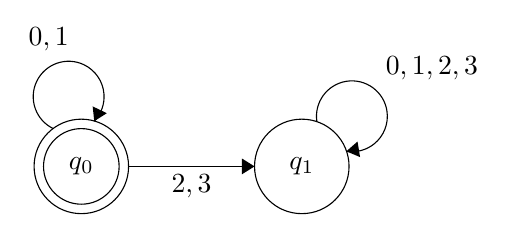
\begin{tikzpicture}[scale=0.2]
            \tikzstyle{every node}+=[inner sep=0pt]
            \draw [black] (25.3,-26.6) circle (3);
            \draw (25.3,-26.6) node {$q_0$};
            \draw [black] (25.3,-26.6) circle (2.4);
            \draw [black] (39.3,-26.6) circle (3);
            \draw (39.3,-26.6) node {$q_1$};
            \draw [black] (23.519,-24.2) arc (244.30485:-43.69515:2.25);
            \draw (23.23,-19.3) node [above] {$0,1$};
            \fill [black] (26.12,-23.73) -- (26.92,-23.22) -- (26.02,-22.79);
            \draw [black] (28.3,-26.6) -- (36.3,-26.6);
            \fill [black] (36.3,-26.6) -- (35.5,-26.1) -- (35.5,-27.1);
            \draw (32.3,-27.1) node [below] {$2,3$};
            \draw [black] (40.26,-23.77) arc (189:-99:2.25);
            \draw (44.6,-20.35) node [right] {$0,1,2,3$};
            \fill [black] (42.13,-25.64) -- (43,-26.01) -- (42.84,-25.02);
            \end{tikzpicture}
        \end{center}
        \item Sum of digits is even. So either 0,2 or even occurrence of 1,3, or these two cases combined.
        \begin{center}
            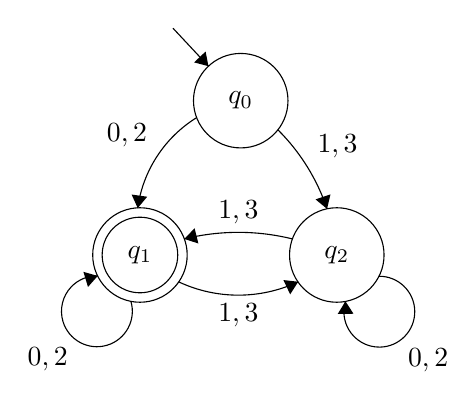
\begin{tikzpicture}[scale=0.2]
                \tikzstyle{every node}+=[inner sep=0pt]
                \draw [black] (31.4,-22.5) circle (3);
                \draw (31.4,-22.5) node {$q_1$};
                \draw [black] (31.4,-22.5) circle (2.4);
                \draw [black] (43.9,-22.5) circle (3);
                \draw (43.9,-22.5) node {$q_2$};
                \draw [black] (37.8,-12.7) circle (3);
                \draw (37.8,-12.7) node {$q_0$};
                \draw [black] (41.447,-24.203) arc (-64.85375:-115.14625:8.936);
                \fill [black] (41.45,-24.2) -- (40.51,-24.09) -- (40.94,-25);
                \draw (37.65,-25.55) node [below] {$1,3$};
                \draw [black] (33.5,-8.1) -- (35.75,-10.51);
                \fill [black] (35.75,-10.51) -- (35.57,-9.58) -- (34.84,-10.27);
                \draw [black] (31.257,-19.521) arc (-187.91981:-238.37418:8.061);
                \fill [black] (31.26,-19.52) -- (31.86,-18.8) -- (30.87,-18.66);
                \draw (31.88,-14.9) node [left] {$0,2$};
                \draw [black] (40.156,-14.547) arc (45.21435:18.58597:12.849);
                \fill [black] (43.28,-19.57) -- (43.5,-18.65) -- (42.55,-18.97);
                \draw (42.64,-15.59) node [right] {$1,3$};
                \draw [black] (34.216,-21.48) arc (103.89644:76.10356:14.3);
                \fill [black] (34.22,-21.48) -- (35.11,-21.77) -- (34.87,-20.8);
                \draw (37.65,-20.56) node [above] {$1,3$};
                \draw [black] (30.823,-25.432) arc (16.59464:-271.40536:2.25);
                \draw (25.54,-28.36) node [below] {$0,2$};
                \fill [black] (28.72,-23.83) -- (27.81,-23.57) -- (28.1,-24.53);
                \draw [black] (46.566,-23.85) arc (90.8699:-197.1301:2.25);
                \draw (49.7,-28.4) node [below] {$0,2$};
                \fill [black] (44.45,-25.44) -- (43.96,-26.24) -- (44.96,-26.23);
                \end{tikzpicture}
            \end{center}
            \item We can accept odd occurrences of 1 and 3, along with any number of 0 or 2 when we have odd 1 and 3. But if we have even occurrences of 1 and 3, along with any nubmer of 0 or 2 in this case, we don't accept.
            \begin{center}
                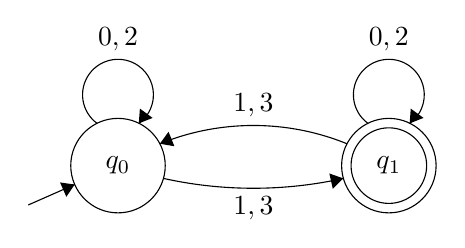
\begin{tikzpicture}[scale=0.2]
                \tikzstyle{every node}+=[inner sep=0pt]
                \draw [black] (46.9,-20.5) circle (3);
                \draw (46.9,-20.5) node {$q_1$};
                \draw [black] (46.9,-20.5) circle (2.4);
                \draw [black] (29.7,-20.5) circle (3);
                \draw (29.7,-20.5) node {$q_0$};
                \draw [black] (32.355,-19.113) arc (112.13204:67.86796:15.78);
                \fill [black] (32.36,-19.11) -- (33.28,-19.27) -- (32.91,-18.35);
                \draw (38.3,-17.45) node [above] {$1,3$};
                \draw [black] (44.014,-21.313) arc (-77.51526:-102.48474:26.432);
                \fill [black] (44.01,-21.31) -- (43.12,-21) -- (43.34,-21.97);
                \draw (38.3,-22.44) node [below] {$1,3$};
                \draw [black] (45.577,-17.82) arc (234:-54:2.25);
                \draw (46.9,-13.25) node [above] {$0,2$};
                \fill [black] (48.22,-17.82) -- (49.1,-17.47) -- (48.29,-16.88);
                \draw [black] (28.377,-17.82) arc (234:-54:2.25);
                \draw (29.7,-13.25) node [above] {$0,2$};
                \fill [black] (31.02,-17.82) -- (31.9,-17.47) -- (31.09,-16.88);
                \draw [black] (24,-23) -- (26.95,-21.7);
                \fill [black] (26.95,-21.7) -- (26.02,-21.57) -- (26.42,-22.48);
                \end{tikzpicture}
            \end{center}
        \end{enumerate}
        \item Worksheet problems (4):
        \begin{enumerate}
            \item We want to remember the last three characters of the string. (Start state $q_0$)
            \begin{center}
                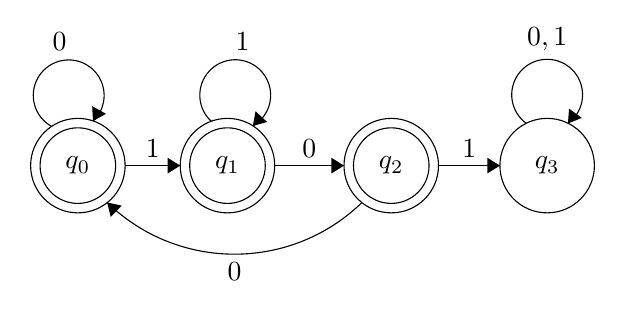
\begin{tikzpicture}[scale=0.2]
                \tikzstyle{every node}+=[inner sep=0pt]
                \draw [black] (23.1,-22.6) circle (3);
                \draw (23.1,-22.6) node {$q_0$};
                \draw [black] (23.1,-22.6) circle (2.4);
                \draw [black] (32.6,-22.6) circle (3);
                \draw (32.6,-22.6) node {$q_1$};
                \draw [black] (32.6,-22.6) circle (2.4);
                \draw [black] (43,-22.6) circle (3);
                \draw (43,-22.6) node {$q_2$};
                \draw [black] (43,-22.6) circle (2.4);
                \draw [black] (52.9,-22.6) circle (3);
                \draw (52.9,-22.6) node {$q_3$};
                \draw [black] (26.1,-22.6) -- (29.6,-22.6);
                \fill [black] (29.6,-22.6) -- (28.8,-22.1) -- (28.8,-23.1);
                \draw (27.85,-22.1) node [above] {$1$};
                \draw [black] (35.6,-22.6) -- (40,-22.6);
                \fill [black] (40,-22.6) -- (39.2,-22.1) -- (39.2,-23.1);
                \draw (37.8,-22.1) node [above] {$0$};
                \draw [black] (46,-22.6) -- (49.9,-22.6);
                \fill [black] (49.9,-22.6) -- (49.1,-22.1) -- (49.1,-23.1);
                \draw (47.95,-22.1) node [above] {$1$};
                \draw [black] (21.442,-20.114) arc (241.43141:-46.56859:2.25);
                \draw (21.93,-15.32) node [above] {$0$};
                \fill [black] (24.06,-19.77) -- (24.89,-19.31) -- (24.01,-18.83);
                \draw [black] (31.579,-19.792) arc (227.71764:-60.28236:2.25);
                \draw (33.56,-15.31) node [above] {$1$};
                \fill [black] (34.21,-20.08) -- (35.12,-19.83) -- (34.38,-19.15);
                \draw [black] (41.14,-24.943) arc (-45.84596:-134.15404:11.614);
                \fill [black] (24.96,-24.94) -- (25.19,-25.86) -- (25.88,-25.14);
                \draw (33.05,-28.72) node [below] {$0$};
                \draw [black] (51.577,-19.92) arc (234:-54:2.25);
                \draw (52.9,-15.35) node [above] {$0,1$};
                \fill [black] (54.22,-19.92) -- (55.1,-19.57) -- (54.29,-18.98);
                \end{tikzpicture}
            \end{center}
        \item Remember the number of times we see 0, and remember every case that we see 1, because we cannot allow more than one 1. (Start state $q_0$)
        \begin{center}
            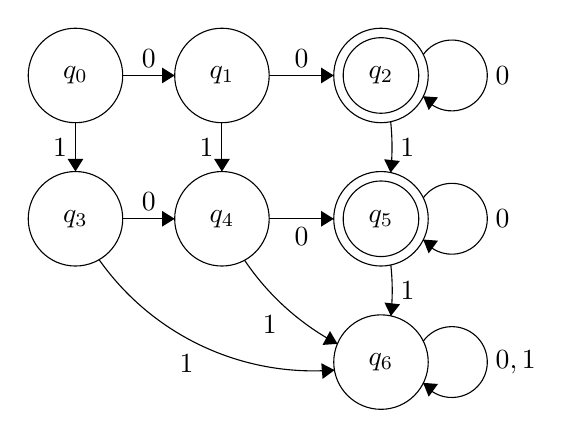
\begin{tikzpicture}[scale=0.2]
            \tikzstyle{every node}+=[inner sep=0pt]
            \draw [black] (23.2,-14.2) circle (3);
            \draw (23.2,-14.2) node {$q_0$};
            \draw [black] (32.5,-14.2) circle (3);
            \draw (32.5,-14.2) node {$q_1$};
            \draw [black] (42.6,-14.2) circle (3);
            \draw (42.6,-14.2) node {$q_2$};
            \draw [black] (42.6,-14.2) circle (2.4);
            \draw [black] (23.2,-23.3) circle (3);
            \draw (23.2,-23.3) node {$q_3$};
            \draw [black] (32.5,-23.3) circle (3);
            \draw (32.5,-23.3) node {$q_4$};
            \draw [black] (42.6,-23.3) circle (3);
            \draw (42.6,-23.3) node {$q_5$};
            \draw [black] (42.6,-23.3) circle (2.4);
            \draw [black] (42.6,-32.4) circle (3);
            \draw (42.6,-32.4) node {$q_6$};
            \draw [black] (26.2,-14.2) -- (29.5,-14.2);
            \fill [black] (29.5,-14.2) -- (28.7,-13.7) -- (28.7,-14.7);
            \draw (27.85,-13.7) node [above] {$0$};
            \draw [black] (35.5,-14.2) -- (39.6,-14.2);
            \fill [black] (39.6,-14.2) -- (38.8,-13.7) -- (38.8,-14.7);
            \draw (37.55,-13.7) node [above] {$0$};
            \draw [black] (43.214,-17.131) arc (6.14405:-6.14405:15.122);
            \fill [black] (43.21,-20.37) -- (43.8,-19.63) -- (42.8,-19.52);
            \draw (43.8,-18.75) node [right] {$1$};
            \draw [black] (43.225,-26.229) arc (6.26737:-6.26737:14.85);
            \fill [black] (43.23,-29.47) -- (43.81,-28.73) -- (42.82,-28.62);
            \draw (43.81,-27.85) node [right] {$1$};
            \draw [black] (45.28,-21.977) arc (144:-144:2.25);
            \draw (49.85,-23.3) node [right] {$0$};
            \fill [black] (45.28,-24.62) -- (45.63,-25.5) -- (46.22,-24.69);
            \draw [black] (45.28,-31.077) arc (144:-144:2.25);
            \draw (49.85,-32.4) node [right] {$0,1$};
            \fill [black] (45.28,-33.72) -- (45.63,-34.6) -- (46.22,-33.79);
            \draw [black] (23.2,-17.2) -- (23.2,-20.3);
            \fill [black] (23.2,-20.3) -- (23.7,-19.5) -- (22.7,-19.5);
            \draw (22.7,-18.75) node [left] {$1$};
            \draw [black] (32.5,-17.2) -- (32.5,-20.3);
            \fill [black] (32.5,-20.3) -- (33,-19.5) -- (32,-19.5);
            \draw (32,-18.75) node [left] {$1$};
            \draw [black] (26.2,-23.3) -- (29.5,-23.3);
            \fill [black] (29.5,-23.3) -- (28.7,-22.8) -- (28.7,-23.8);
            \draw (27.85,-22.8) node [above] {$0$};
            \draw [black] (35.5,-23.3) -- (39.6,-23.3);
            \fill [black] (39.6,-23.3) -- (38.8,-22.8) -- (38.8,-23.8);
            \draw (37.55,-23.8) node [below] {$0$};
            \draw [black] (39.836,-31.245) arc (-117.94623:-146.09085:16.33);
            \fill [black] (39.84,-31.24) -- (39.36,-30.43) -- (38.89,-31.31);
            \draw (35.54,-29.44) node [below] {$1$};
            \draw [black] (39.647,-32.906) arc (-85.42866:-144.83127:16.662);
            \fill [black] (39.65,-32.91) -- (38.81,-32.47) -- (38.89,-33.47);
            \draw (30.26,-31.89) node [below] {$1$};
            \draw [black] (45.28,-12.877) arc (144:-144:2.25);
            \draw (49.85,-14.2) node [right] {$0$};
            \fill [black] (45.28,-15.52) -- (45.63,-16.4) -- (46.22,-15.59);
            \end{tikzpicture}
        \end{center}
        \item When we see a 1, we cannot allow any 0 to occur (\textit{dump state} $q_2$). This one is the tricky.
        \begin{center}
            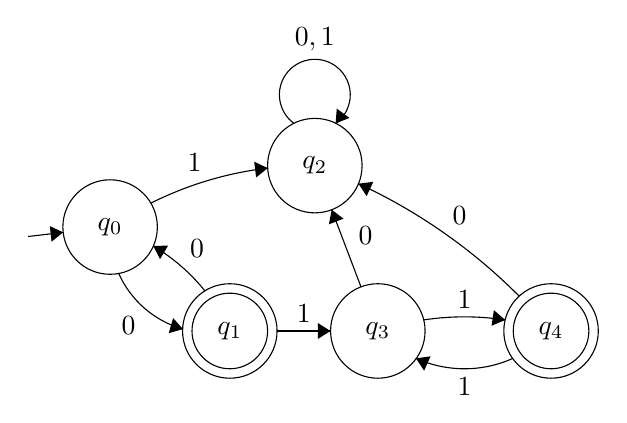
\begin{tikzpicture}[scale=0.2]
                \tikzstyle{every node}+=[inner sep=0pt]
                \draw [black] (20.3,-23.2) circle (3);
                \draw (20.3,-23.2) node {$q_0$};
                \draw [black] (27.9,-29.8) circle (3);
                \draw (27.9,-29.8) node {$q_1$};
                \draw [black] (27.9,-29.8) circle (2.4);
                \draw [black] (33.3,-19.3) circle (3);
                \draw (33.3,-19.3) node {$q_2$};
                \draw [black] (37.3,-29.8) circle (3);
                \draw (37.3,-29.8) node {$q_3$};
                \draw [black] (48.3,-29.8) circle (3);
                \draw (48.3,-29.8) node {$q_4$};
                \draw [black] (48.3,-29.8) circle (2.4);
                \draw [black] (24.93,-29.68) arc (-105.78843:-156.15505:6.374);
                \fill [black] (24.93,-29.68) -- (24.3,-28.98) -- (24.02,-29.94);
                \draw (21.47,-28.85) node [below] {$0$};
                \draw [black] (23.039,-24.405) arc (59.24686:38.80967:12.258);
                \fill [black] (23.04,-24.4) -- (23.47,-25.24) -- (23.98,-24.38);
                \draw (25.82,-25.19) node [above] {$0$};
                \draw [black] (22.885,-21.683) arc (116.59491:96.80358:22.541);
                \fill [black] (30.31,-19.46) -- (29.45,-19.05) -- (29.57,-20.05);
                \draw (25.66,-19.7) node [above] {$1$};
                \draw [black] (31.977,-16.62) arc (234:-54:2.25);
                \draw (33.3,-12.05) node [above] {$0,1$};
                \fill [black] (34.62,-16.62) -- (35.5,-16.27) -- (34.69,-15.68);
                \draw [black] (30.9,-29.8) -- (34.3,-29.8);
                \fill [black] (34.3,-29.8) -- (33.5,-29.3) -- (33.5,-30.3);
                \draw (32.6,-29.3) node [above] {$1$};
                \draw [black] (40.213,-29.097) arc (98.59852:81.40148:17.305);
                \fill [black] (45.39,-29.1) -- (44.67,-28.48) -- (44.52,-29.47);
                \draw (42.8,-28.4) node [above] {$1$};
                \draw [black] (45.88,-31.539) arc (-65.7562:-114.2438:7.501);
                \fill [black] (39.72,-31.54) -- (40.24,-32.32) -- (40.65,-31.41);
                \draw (42.8,-32.7) node [below] {$1$};
                \draw [black] (36.072,-20.446) arc (65.11855:44.89741:35.473);
                \fill [black] (36.07,-20.45) -- (36.59,-21.24) -- (37.01,-20.33);
                \draw (42.49,-23.07) node [above] {$0$};
                \draw [black] (36.23,-27) -- (34.37,-22.1);
                \fill [black] (34.37,-22.1) -- (34.19,-23.03) -- (35.12,-22.67);
                \draw (36.05,-23.72) node [right] {$0$};
                \draw [black] (15.1,-23.8) -- (17.32,-23.54);
                \fill [black] (17.32,-23.54) -- (16.47,-23.14) -- (16.58,-24.13);
                \end{tikzpicture}
        \end{center}
    \end{enumerate}
\end{enumerate}
    

\end{document}



